\section{Conjuntos de Dados}

\subsection{Sintéticos}

\subsubsection*{Estacionários}

Estáticos 2D \autoref{Fig:SinteticosEstaticos}.

set.seed(1000)

gerador R: Barras e Gaussianas com 10000 exemplos - A data stream generator which creates the shape of two bars and two Gaussians clusters with different density. Conjunto BG\_10k, \autoref{Fig:BarGauss}.

gerador R: Mistura de Gaussianas - A data stream generator that produces a data stream with a mixture of static Gaussians

3 Gaussianas em 2 dimensões com 10000 exemplos. Conjunto MGK3D2\_10k, \autoref{Fig:GaussK3D2}.

4 Gaussianas em 2 dimensões com 10000 exemplos. Conjunto MGK4D2\_10k, \autoref{Fig:GaussK4D2}.

\begin{figure}[!htb]
        \centering
        \begin{subfigure}[t]{0.4\textwidth}
                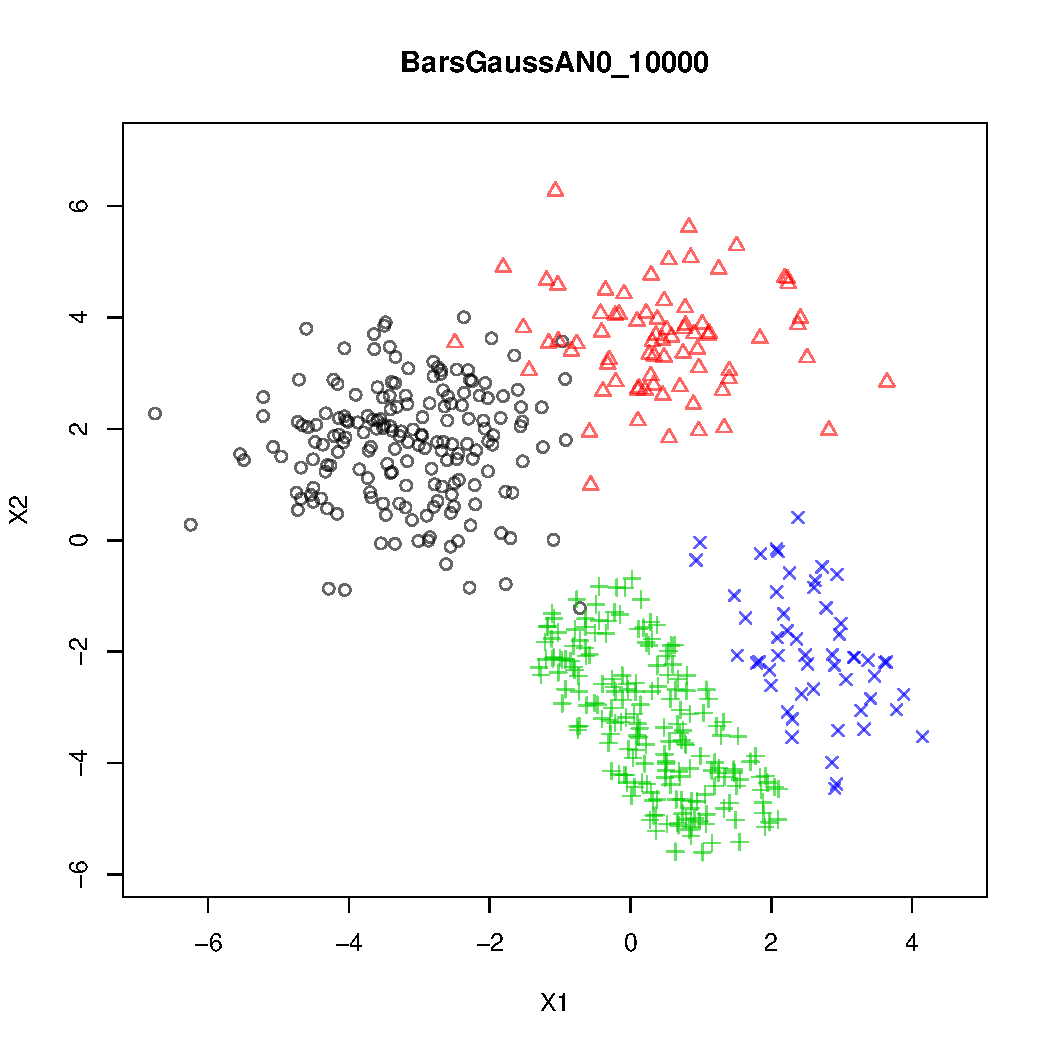
\includegraphics[width=\textwidth]{figures/datasets/BarsGaussAN0_10000}
                \caption{BG\_10k}
                \label{Fig:BarGauss}
        \end{subfigure}%
        \qquad %add desired spacing between images, e. g. ~, \quad, \qquad, \hfill etc.
          %(or a blank line to force the subfigure onto a new line)
        \begin{subfigure}[t]{0.4\textwidth}
                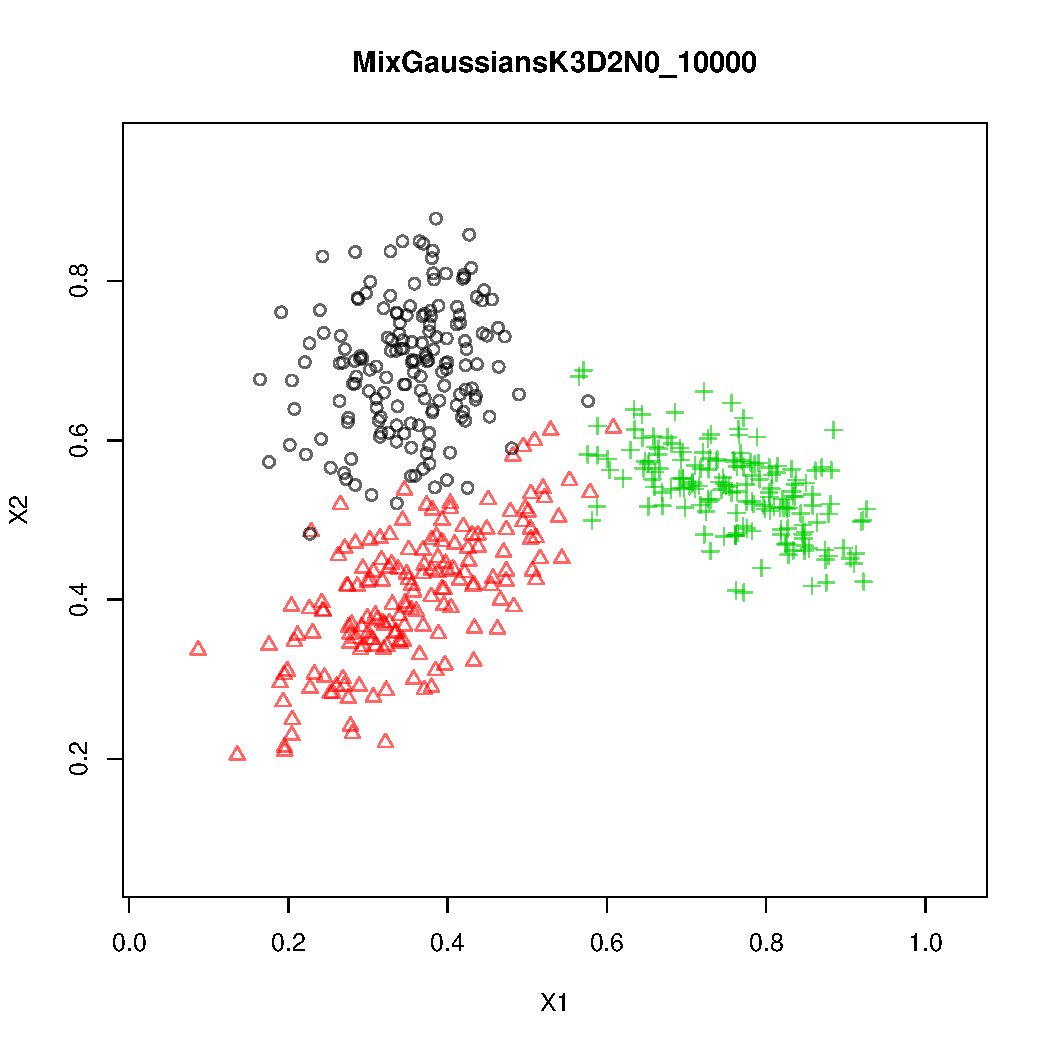
\includegraphics[width=\textwidth]{figures/datasets/MixGaussiansK3D2N0_10000}
                \caption{MGK3D2\_10k}
                \label{Fig:GaussK3D2}
        \end{subfigure}
        \qquad %add desired spacing between images, e. g. ~, \quad, \qquad, \hfill etc.
        %(or a blank line to force the subfigure onto a new line)
        \begin{subfigure}[t]{0.4\textwidth}
                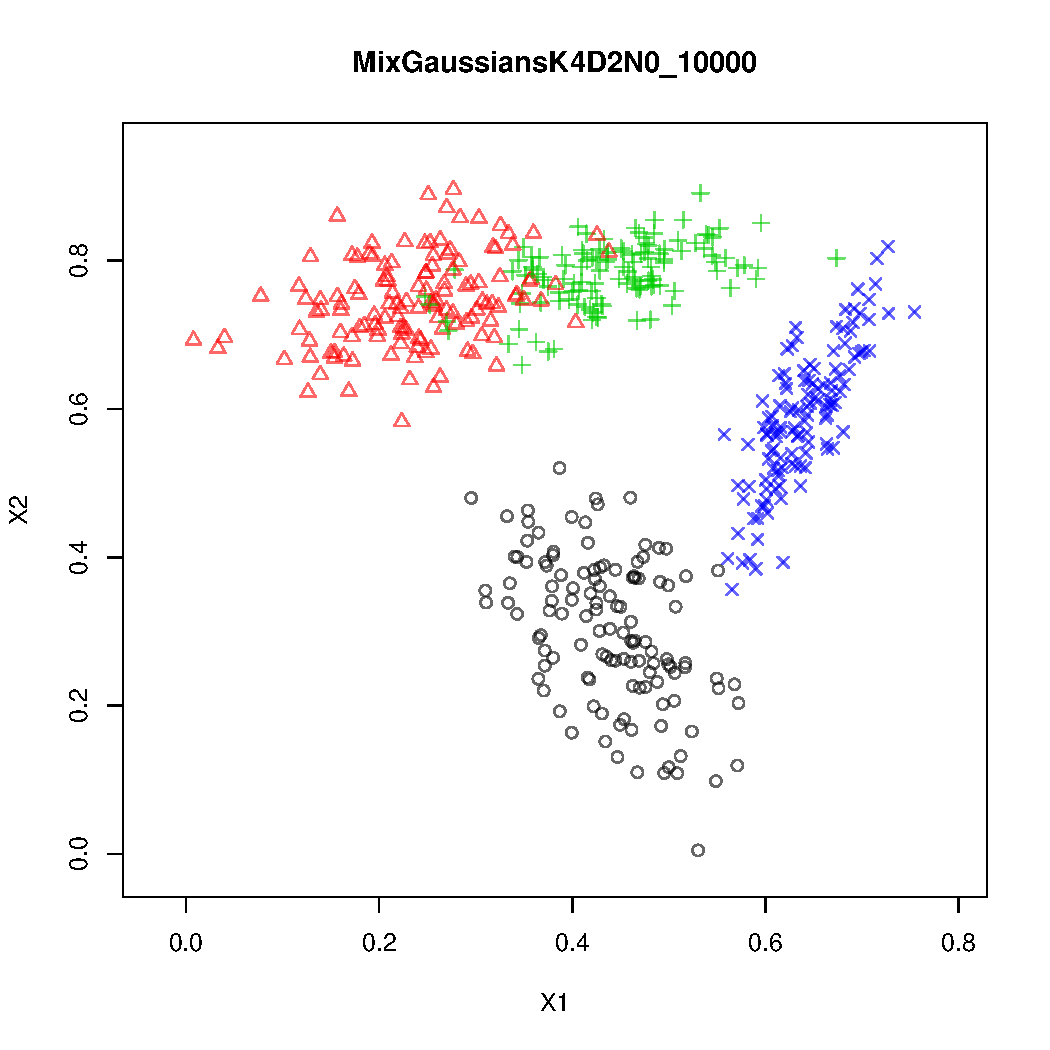
\includegraphics[width=\textwidth]{figures/datasets/MixGaussiansK4D2N0_10000}
                \caption{MGK4D2\_10k}
                \label{Fig:GaussK4D2}
        \end{subfigure}
        \caption{Gráficos 500 pares de exemplos de cada conjunto BG\_10k, MGK3D2\_10k e MGK4D2\_10k}\label{Fig:SinteticosEstaticos}
\end{figure}

Mistura de 3 Gaussianas em 3 dimensões com 10000 exemplos. Conjunto MGK3D3\_10k, \autoref{Fig:GaussK3D3}.

\subsubsection*{Não Estacionários}

gerador R: DSD\_Benchmark(i) - A data stream generator that generates several dynamic streams indented to be benchmarks to compare data stream clustering algorithms. Available: $i = 1$ e $i = 2$.

DSD\_Benchmark(1) - creates two clusters moving in two-dimensional space. One moves from top left to bottom right and the other one moves from bottom left to top right. Both clusters overlap when they meet exactly in the center of the data space.

Com 5500 exemplos. Conjunto GB1\_5.5k \autoref{Fig:Benchmark1}.

\begin{figure}[!htb]
        \centering
        \begin{subfigure}[t]{0.25\textwidth}
                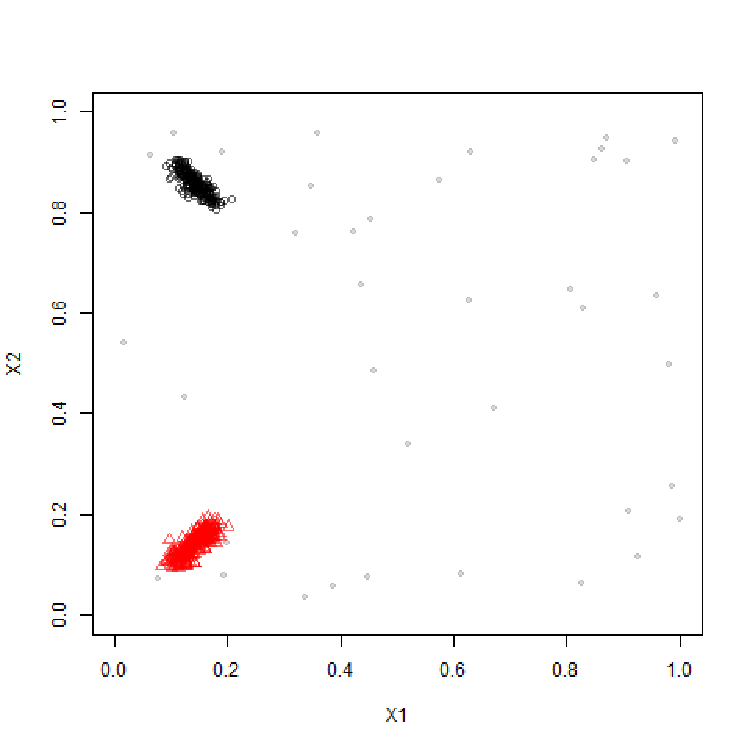
\includegraphics[page=1,width=\textwidth]{figures/datasets/Benchmark1_5500}
                \caption{$t = 0$}
                \label{Fig:Benchmark1_11}
        \end{subfigure}%
        \qquad %add desired spacing between images, e. g. ~, \quad, \qquad, \hfill etc.
          %(or a blank line to force the subfigure onto a new line)
%        \begin{subfigure}[t]{0.25\textwidth}
%                \includegraphics[page=3,width=\textwidth]{figures/datasets/Benchmark1_5500}
%                \caption{$t = 2$}
%                \label{Fig:Benchmark1_12}
%        \end{subfigure}%
%        \qquad %add desired spacing between images, e. g. ~, \quad, \qquad, \hfill etc.
        %(or a blank line to force the subfigure onto a new line)
        \begin{subfigure}[t]{0.25\textwidth}
                \includegraphics[page=5,width=\textwidth]{figures/datasets/Benchmark1_5500}
                \caption{$t = 4$}
                \label{Fig:Benchmark1_13}
        \end{subfigure}%
		\qquad %add desired spacing between images, e. g. ~, \quad, \qquad, \hfill etc.
        %(or a blank line to force the subfigure onto a new line)
        \begin{subfigure}[t]{0.25\textwidth}
                \includegraphics[page=6,width=\textwidth]{figures/datasets/Benchmark1_5500}
                \caption{$t = 5$}
                \label{Fig:Benchmark1_14}
        \end{subfigure}%
		\qquad %add desired spacing between images, e. g. ~, \quad, \qquad, \hfill etc.
        %(or a blank line to force the subfigure onto a new line)
        \begin{subfigure}[t]{0.25\textwidth}
                \includegraphics[page=7,width=\textwidth]{figures/datasets/Benchmark1_5500}
                \caption{$t = 6$}
                \label{Fig:Benchmark1_15}
        \end{subfigure}%
        \qquad %add desired spacing between images, e. g. ~, \quad, \qquad, \hfill etc.
        %(or a blank line to force the subfigure onto a new line)
%        \begin{subfigure}[t]{0.25\textwidth}
%                \includegraphics[page=9,width=\textwidth]{figures/datasets/Benchmark1_5500}
%                \caption{$t = 8$}
%                \label{Fig:Benchmark1_16}
%        \end{subfigure}%
%		\qquad %add desired spacing between images, e. g. ~, \quad, \qquad, \hfill etc.
        %(or a blank line to force the subfigure onto a new line)
        \begin{subfigure}[t]{0.25\textwidth}
                \includegraphics[page=11,width=\textwidth]{figures/datasets/Benchmark1_5500}
                \caption{$t = 10$}
                \label{Fig:Benchmark1_17}
        \end{subfigure}%
		\caption{500 exemplos do conjunto GB1\_5.5k em diferentes tempos $t$}\label{Fig:Benchmark1}
\end{figure}

\rewrite{
Benchmark1 com 11000 exemplos (vai e volta) - se eu conseguir rodar

DSD\_Benchmark(2) - ver qual o comportamento

DSD\_MG, a generator to specify complex data streams with concept drift. The shape as well as the behavior of each cluster over time (changes in position, density and dispersion) can be specified using keyframes (similar to keyframes in animation and film making) or by mathematical functions.

DSD\_RandomRBFGeneratorEvents (streamMOA) generates streams using radial base functions with noise. Clusters move, merge and split.
}

\subsection{Benchmark}

\begin{itemize}
    \item KDDCup 99
    \item Forest Covertype
\end{itemize}